\part{Novell Open Enterprise Server 2}
Novell OES2 представляет собой законченное решение по предоставлению базовых сетевых сервисов - регистрация пользователей в сети, сетевая печать, порталы доступа и управления. OES2 может заменить собой любую из существующих систем на базе Linux/Netware/Windows, а присутствующий инструменты миграции обеспечат плавную миграцию данных. Решение построено на базе открытой платформы SUSE Linux Enterprise Server 10 (SLES10) с добавлением функционала коммерческих сервисов Novell. Весомым преимуществом решения можно назвать его высокую степень интегрированности и веб-ориентированности. Управления сетью OES2 сильно проще и удобнее чем даже Windows, а гибкость настройки не ниже чем у любой Linux-системы.

\section{Получение дистрибутива}
Как уже говорилось, решение построено на базе SLES10. Соответственно для установки нам в первую очередь потребуется этот дистрибутив. Дополнительные сервисы вынесены в отдельный диск, функционально являющийся Add-on для SLES10.\par
Чтобы скачать все необходимые пакеты необходимо зарегистрироваться на портале www.novell.com (регистрация бесплатна).\par
Последнюю версию OES2 можно найти на странице novell.com\footnote{http://www.novell.com/products/openenterpriseserver/}. Для установки потребуется скачать SLES10 (32 или 64-битную платформу). Плюс к этому скачиваем диск начинающийся на OES2 (соответственно выбранной платформе).\\
\clearpage

\section{Установка}
Начало установки.\par
Установка начинается с загрузки сервера с диска SLES10 DVD1. Диск с сервисами OES2 пригодится несколько позже, во время настройки. Если загрузка удалась, то вы увидите следующее окно. (рис.~\ref{fig1})
\begin{figure}[H]
\center{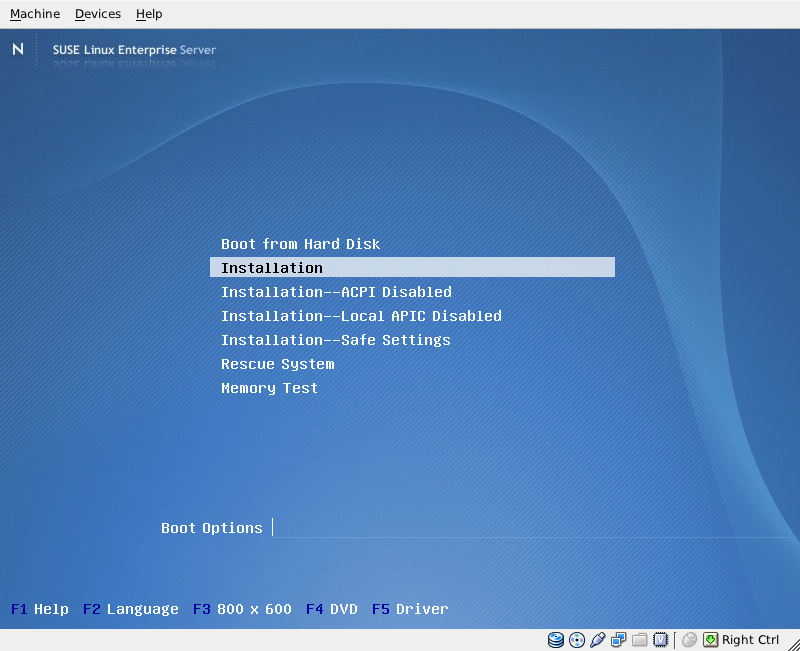
\includegraphics[width=1\linewidth]{oes/1.png}}
\caption{Начало установки}
\label{fig1}
\end{figure}
По умолчанию выбран пункт <<Boot from Hard Disk>> (Загрузка с жёсткого диска). Для начала установки выбираем пункт <<Installation>>.
\clearpage

Первое окно — выбор языка установки, выбираем <<Русский>>, нажимаем <<Применить>>. (рис.~\ref{fig2})
\begin{figure}[H]
\center{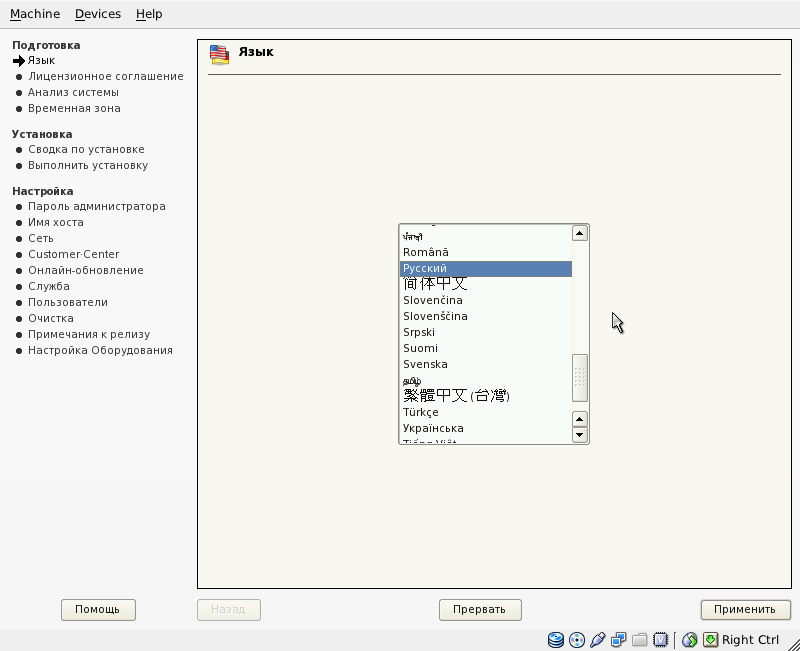
\includegraphics[width=1\linewidth]{oes/2.png}}
\caption{Выбор языка}
\label{fig2}
\end{figure}
\clearpage

Далее предлагается принять лицензию на SLES10 <<Да, я согласен с условиями лицензионного соглашения>>, без чего дальнейшая установка невозможна. (рис.~\ref{fig3})
\begin{figure}[H]
\center{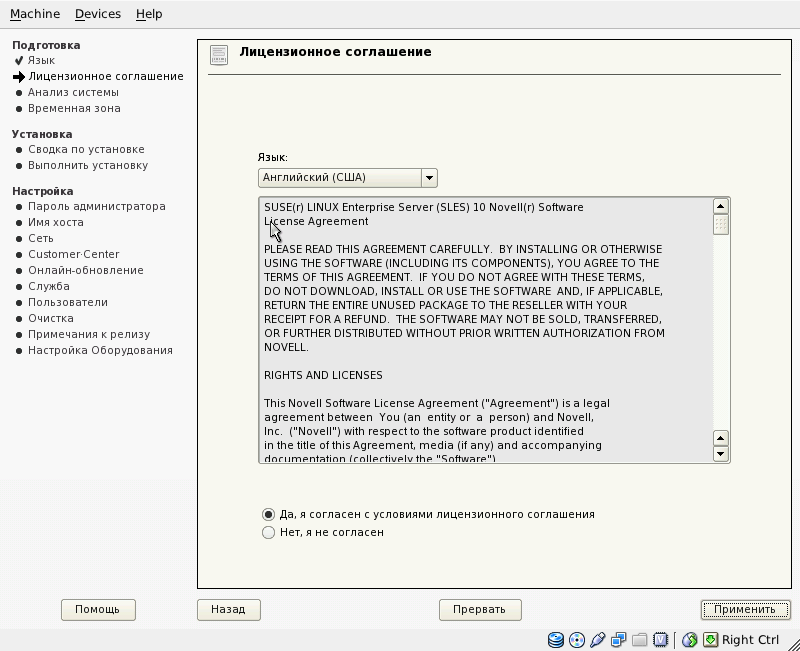
\includegraphics[width=1\linewidth]{oes/3.png}}
\caption{Лицензионное соглашение}
\label{fig3}
\end{figure}
\clearpage

Установщик автоматически предлагает вариант <<Новая установка>>. Если бы на сервере была установлена какой-либо SUSE Linux, то был бы доступен выбор варианта обновления. (рис.~\ref{fig4})
\begin{figure}[H]
\center{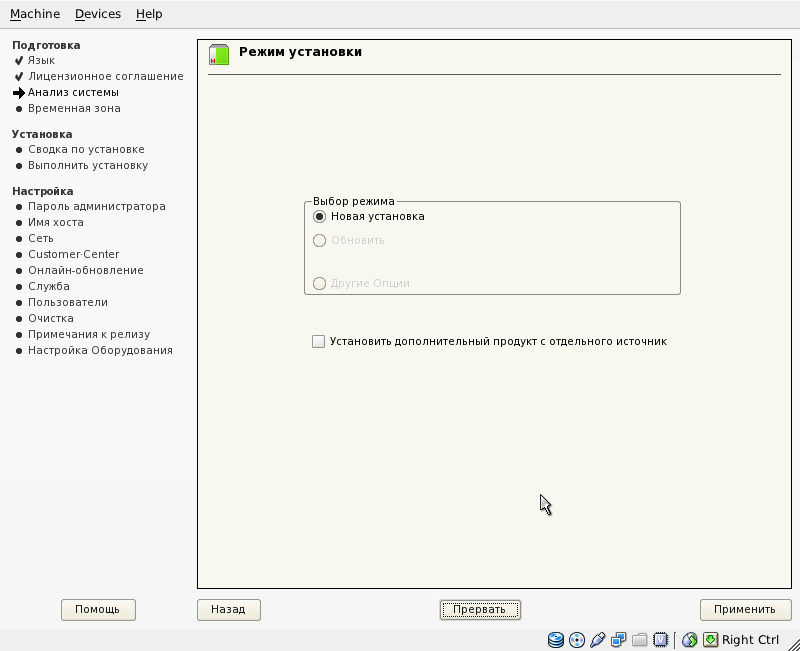
\includegraphics[width=1\linewidth]{oes/4.png}}
\caption{Выбор режима установки}
\label{fig4}
\end{figure}
\clearpage

После выбора временной зоны появляется итоговая сводка. Это последний этап конфигурирования системы перед установкой. На последующих шагах для настройки NSS\footnote{Novell Storage Services (NSS) - файловая система, используемая в Novell для создания томов на файловом сервере} нам потребуется свободное дисковое пространство. Для этого можно выделить отдельный жесткий диск (или же поднять для этих целей отдельностоящий сервер). В нашем случае мы переразобъём текущий раздел, выделив свободное место на нём.
\begin{figure}[H]
\center{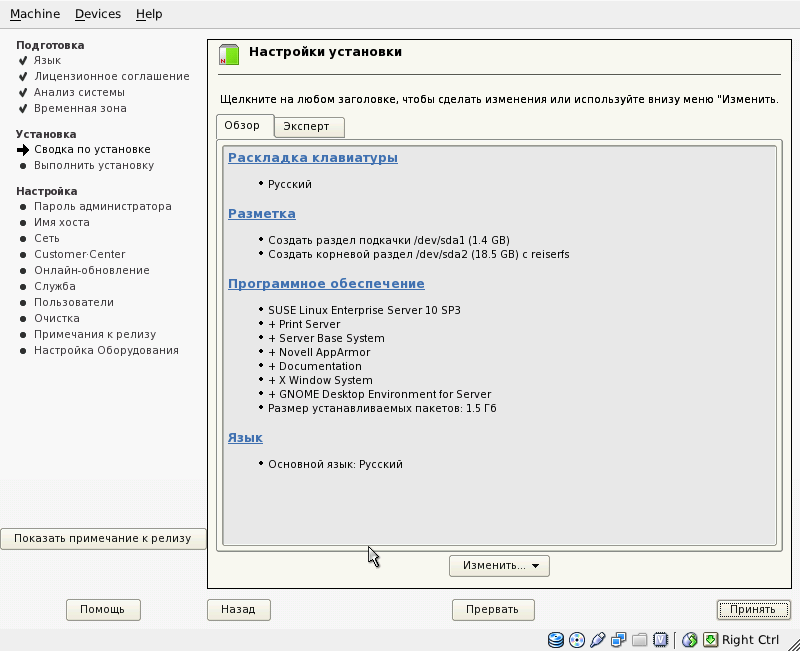
\includegraphics[width=1\linewidth]{oes/p1.png}}
\caption{Сводка установки}
\label{p1}
\end{figure}
Заходим в раздел <<Разметка>>.
\clearpage

Полностью переделывать разметку мы не будем, поэтому выбираем пункт <<Настроить раздел согласно предложению>>.
\begin{figure}[H]
\center{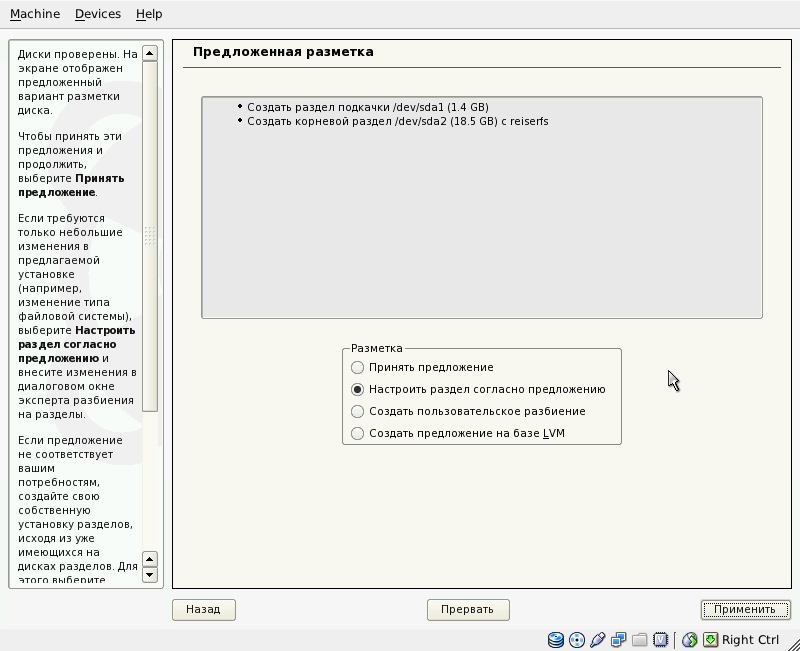
\includegraphics[width=1\linewidth]{oes/p2.png}}
\caption{Предложенная разметка}
\label{p2}
\end{figure}
\clearpage

Здесь мы уменьшим основной раздел нажав кнопку <<Изменить размер>>.
\begin{figure}[H]
\center{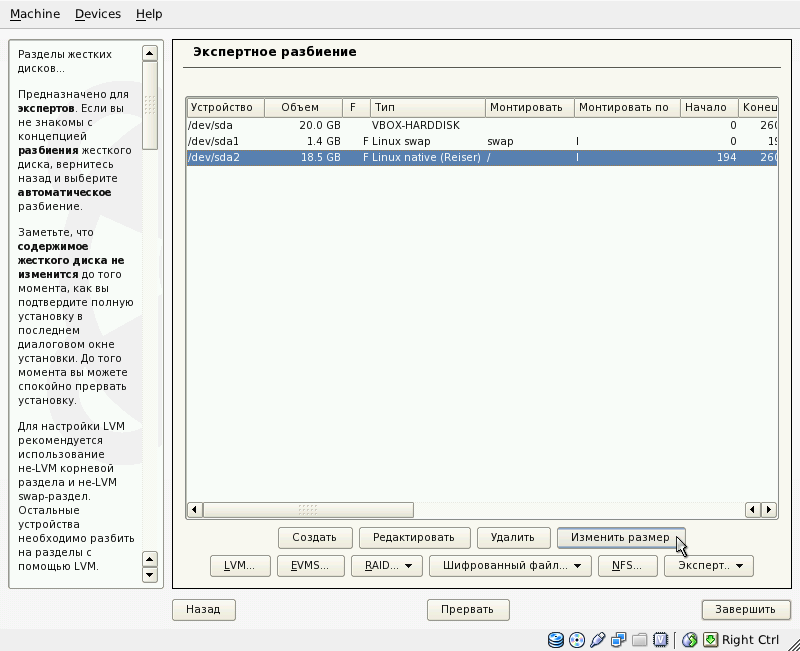
\includegraphics[width=1\linewidth]{oes/p3.png}}
\caption{Изменение разметки}
\label{p3}
\end{figure}
\clearpage

Отрезаем часть от раздела. В будущем мы используем это свободное пространство для создания NSS томов.
\begin{figure}[H]
\center{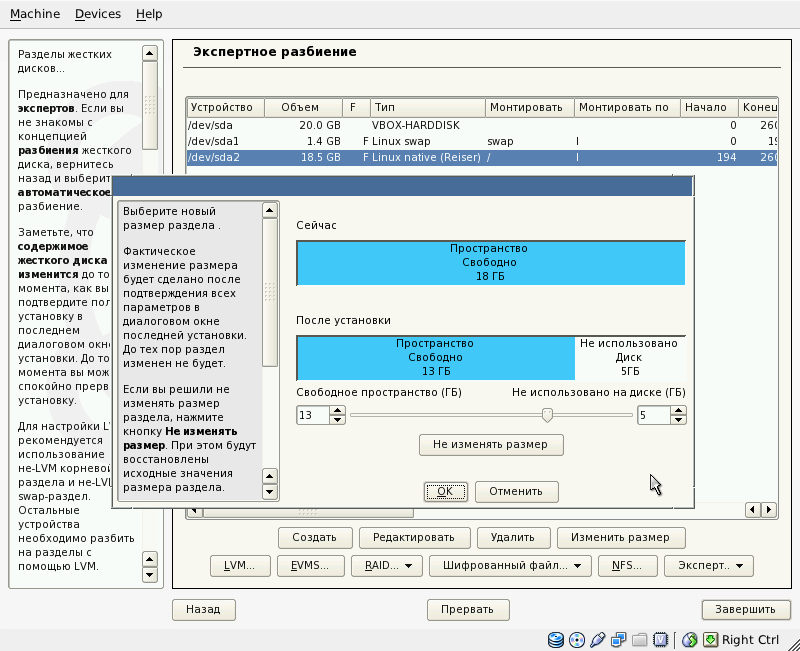
\includegraphics[width=1\linewidth]{oes/p4.png}}
\caption{Изменение разметки}
\label{p4}
\end{figure}
\clearpage

Теперь у нас появилось немного свободного дискового пространства, можно приступать к установке, нажав <<Принять>>. (рис.~\ref{p5})
\begin{figure}[H]
\center{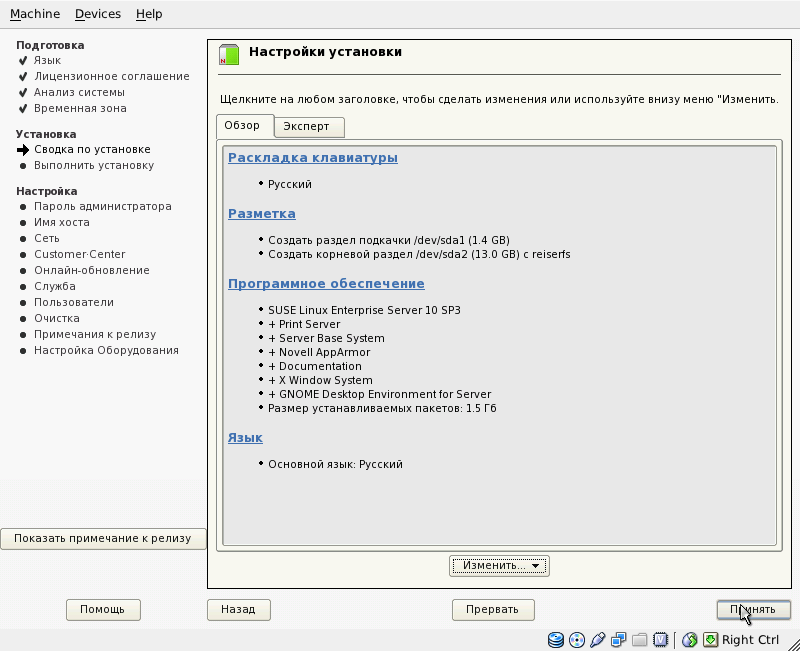
\includegraphics[width=1\linewidth]{oes/p5.png}}
\caption{Сводка установки}
\label{p5}
\end{figure}
\clearpage

После перезагрузки мы можем приступить к первоначальной настройке сервера.\\
Начинаем с пароля администратора root. Если пароль указать недостаточно стойким или присутствующим в базе типовых паролей, то система выдаст предупреждение о потенциальной угрозе. (рис.~\ref{fig6})
\begin{figure}[H]
\center{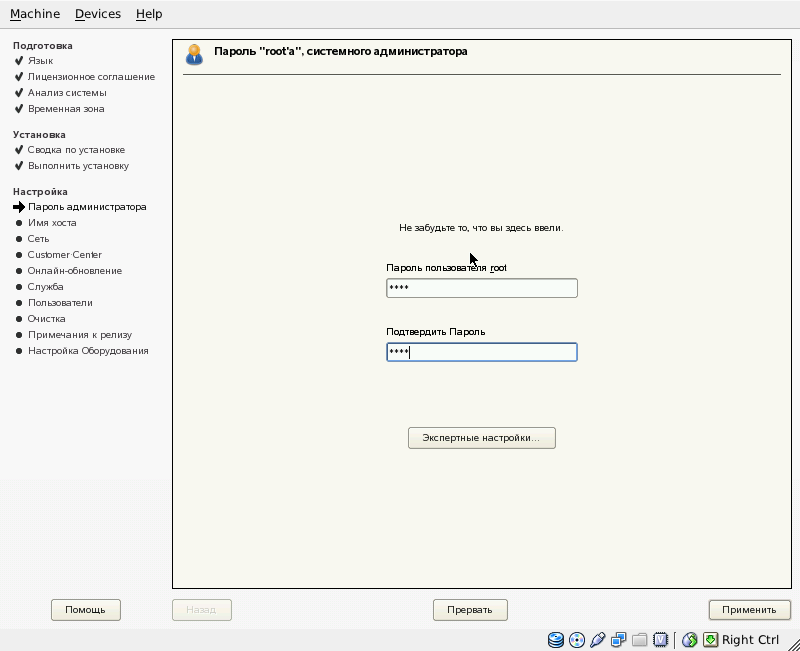
\includegraphics[width=1\linewidth]{oes/rootpasswd.png}}
\caption{Пароль системного администратора}
\label{fig6}
\end{figure}
\clearpage

Следующий этап это указание имени узла (в нашем случае oes2 - по названию операционной системы) и домена DNS (вариации на тему <имя компании>.ru). (рис.~\ref{fig7})
\begin{figure}[H]
\center{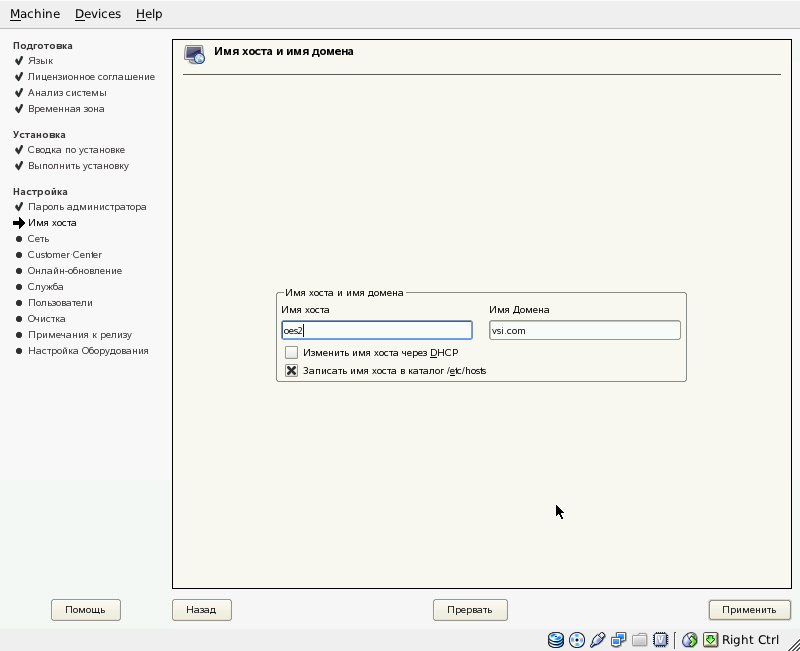
\includegraphics[width=1\linewidth]{oes/7.png}}
\caption{Имя хоста и имя домена}
\label{fig7}
\end{figure}
\clearpage

В разделе <<Настройка сети>> необходимо задать ip адрес сервера. По умолчанию сетевые адаптеры не настроены, либо настроены на использование DHCP, что совершенно не годится в случае с сервером. Для этого нажимаем <<Изменить>> и выбираем <<Сетевые интерфейсы>> (рис.~\ref{figNetworkall})
\begin{figure}[H]
\center{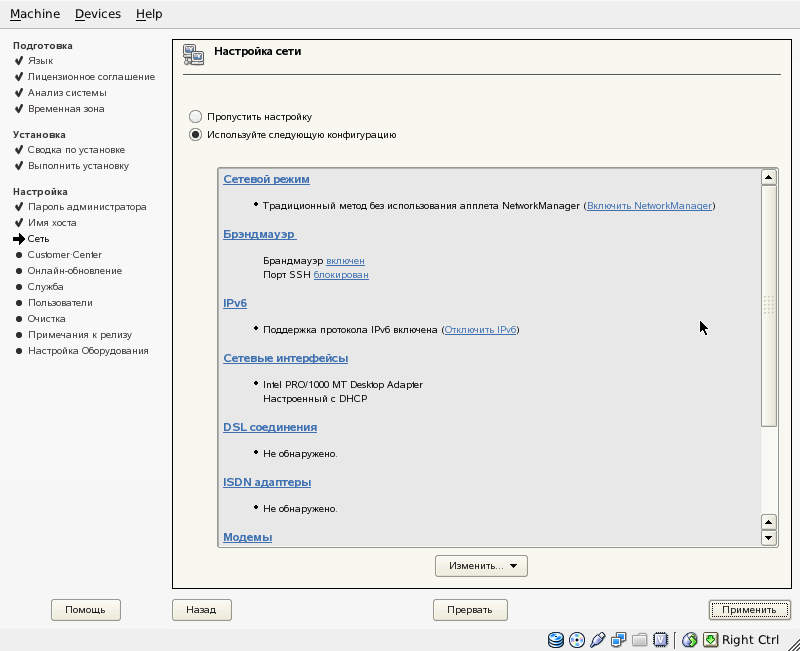
\includegraphics[width=1\linewidth]{oes/networkall.png}}
\caption{Настройка сети}
\label{figNetworkall}
\end{figure}
\clearpage

Сетевую карту необходимо настроить на статическое получение адреса — выбрать <<Установка статического адреса>> и задать все необходимые параметры: IP-адрес и маску подсети.
\begin{figure}[H]
\center{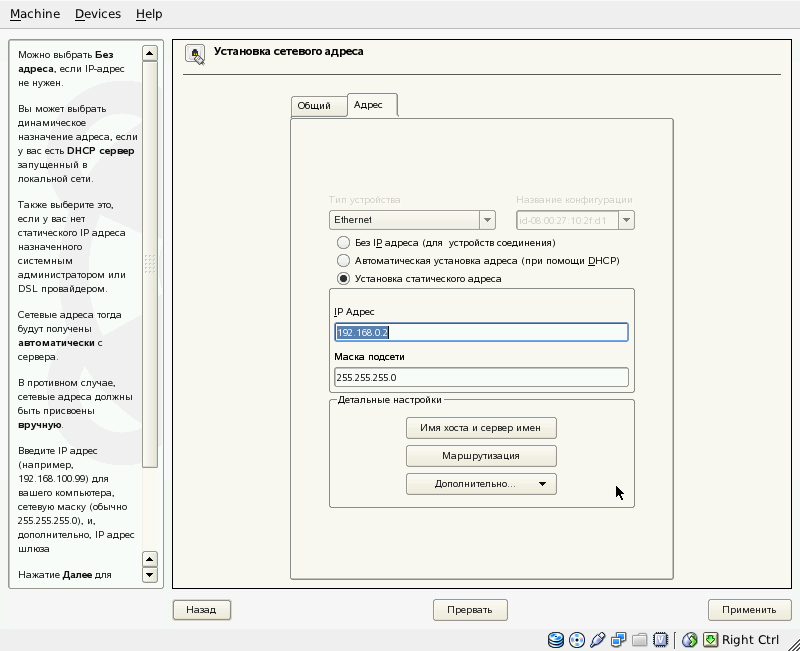
\includegraphics[width=1\linewidth]{oes/8.png}}
\caption{Настройка сетевого адреса}
\label{fig8}
\end{figure}
\clearpage

Следующим шагом будет настройка DNS. Жмём <<Имя хоста и сервер имён>> и прописываем наш сервер в <<Сервер имён 1>>. Завершаем настройку кнопкой <<Применить>>. (рис.~\ref{fig9})
\begin{figure}[H]
\center{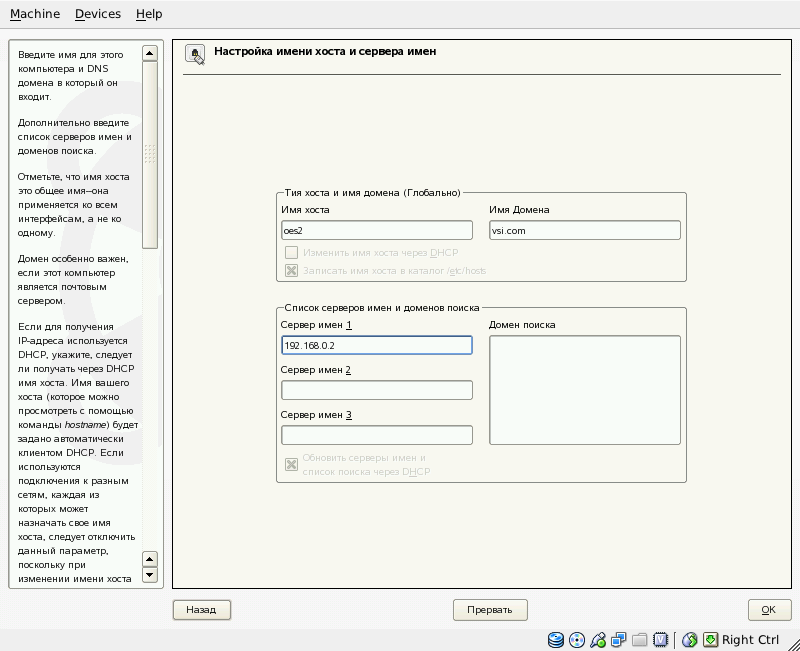
\includegraphics[width=1\linewidth]{oes/9.png}}
\caption{Настройка DNS}
\label{fig9}
\end{figure}
\clearpage

Теперь, когда сеть настроена, можно попробовать подключиться к сети Интернет и проверить последние обновления с сайта novell.com. (рис.~\ref{fig10})
\begin{figure}[H]
\center{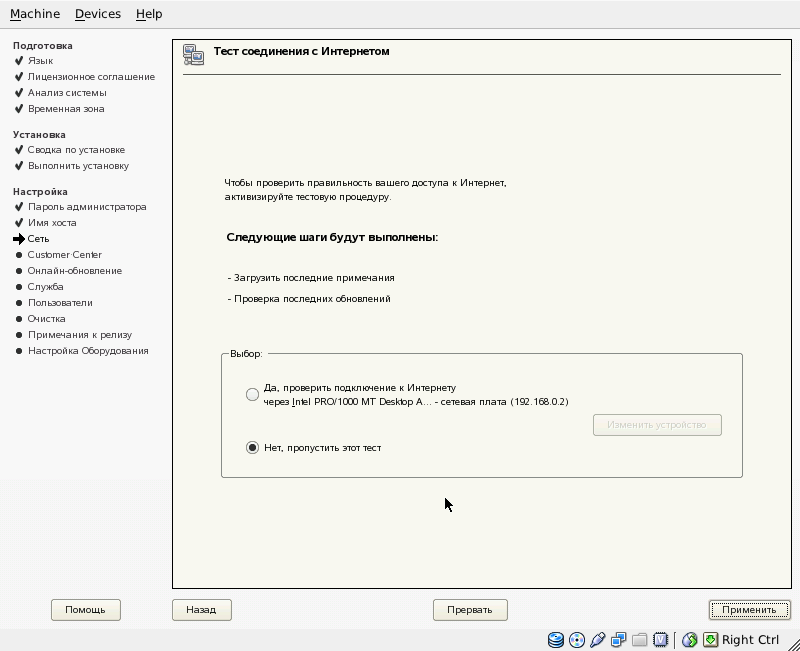
\includegraphics[width=1\linewidth]{oes/10.png}}
\caption{Тест соединения с Интернетом}
\label{fig10}
\end{figure}
Если на текущем этапе нет желания или возможности проверить подключение к сети Интернет, то выбираем вариант <<Нет, пропустить этот тест>>.
\clearpage

Добавить скрин с сертификатом.
\clearpage

Ещё один тонкий момент, требующий внимания — настройка сертификата сервера. Как видно исходное значения поля <<Страна>> выставлено равным <<RU.KOI8-R>>, что не совсем правильно. Чтобы изменить параметры сертификата жмём линк <<Управление СА>>. В открывшемся окне находим кнопку <<Редактировать Установки по Умолчанию>> и меняем поле страна на Россия. (рис.~\ref{fig11})
\begin{figure}[H]
\center{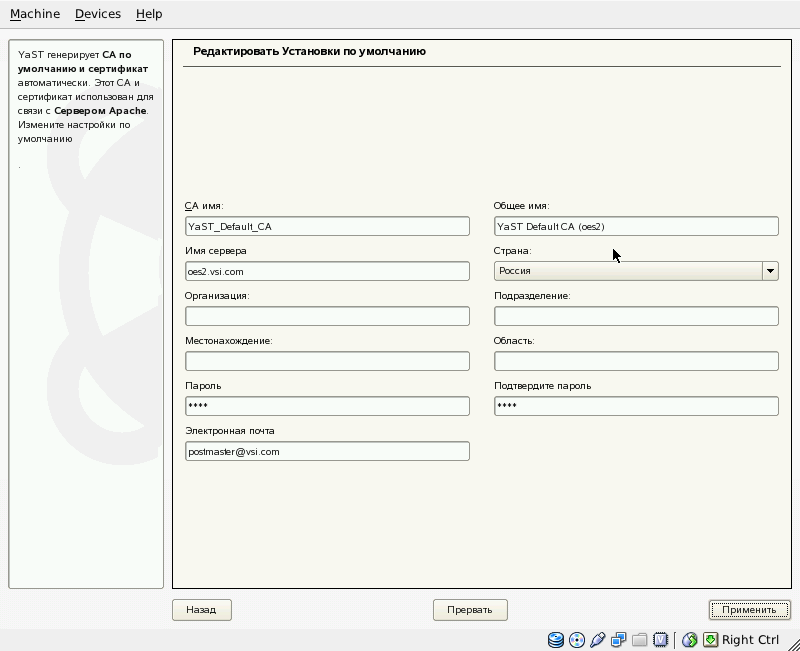
\includegraphics[width=1\linewidth]{oes/11.png}}
\caption{Редактирование CA сертификата}
\label{fig11}
\end{figure}
\clearpage

Следующий этап это создание локальных пользователей. (рис.~\ref{fig12})
\begin{figure}[H]
\center{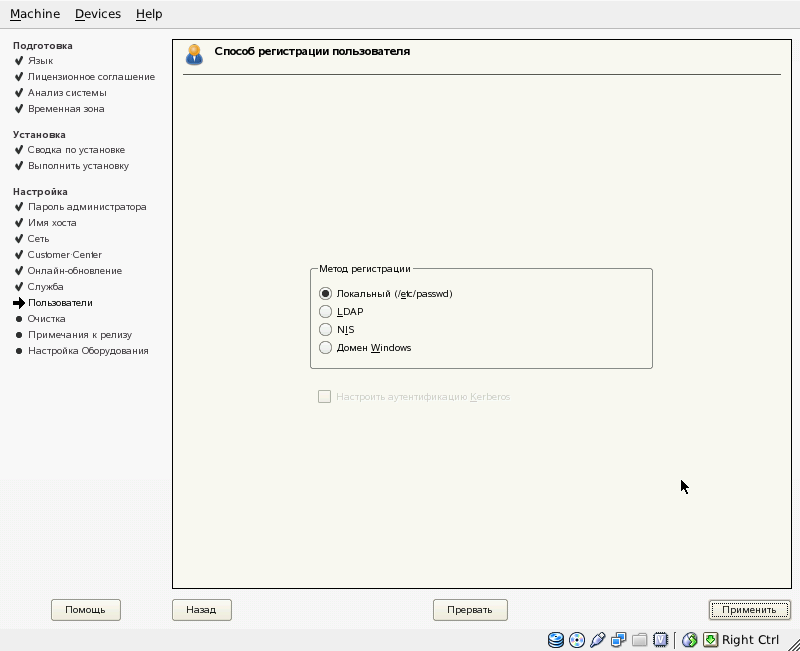
\includegraphics[width=1\linewidth]{oes/12.png}}
\caption{Способ регистрации пользователей}
\label{fig12}
\end{figure}
Выбираем метод регистрации <<Локальный (/etc/passwd)>>.
\clearpage

Произвольно задаём имя пользователя и пароль. (рис.~\ref{fig13})
\begin{figure}[H]
\center{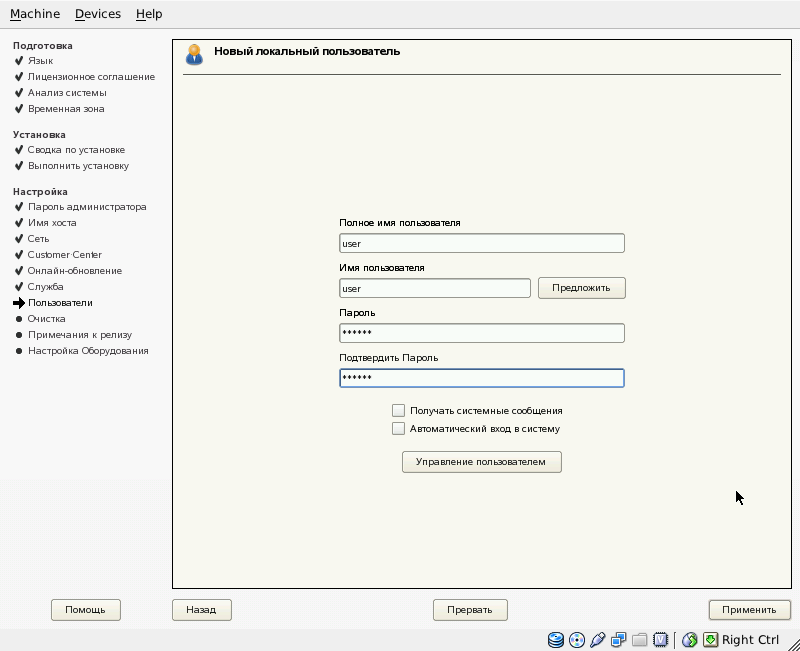
\includegraphics[width=1\linewidth]{oes/13.png}}
\caption{Создание локального пользователя}
\label{fig13}
\end{figure}
Жмём кнопку <<Применить>>, переходим к окну примечаний к выпуску и вновь жмём кнопку <<Применить>>.
\clearpage

Окно настройки оборудования показывает текущие настройки видеокарты, принтеров и звука. Оставляем всё без изменений. (рис.~\ref{fig14})
\begin{figure}[H]
\center{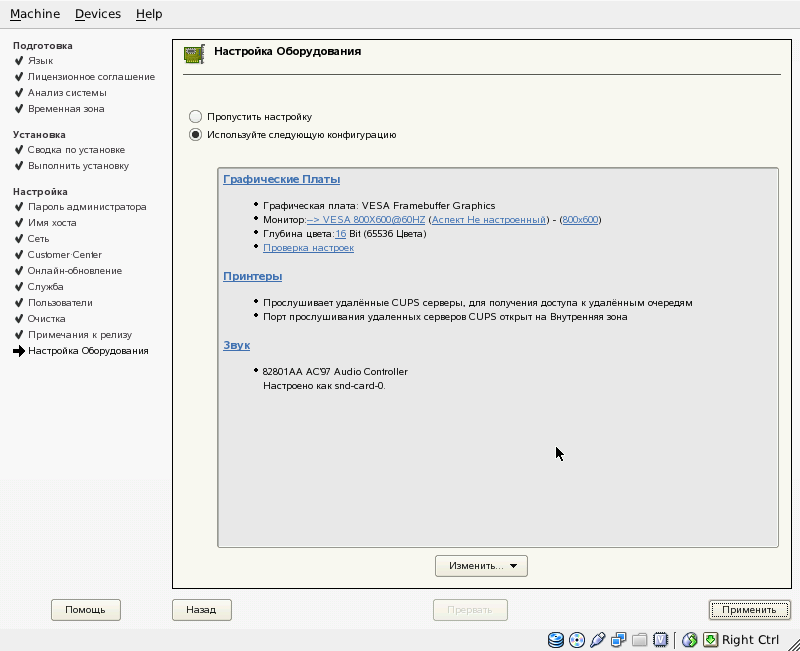
\includegraphics[width=1\linewidth]{oes/14.png}}
\caption{Настройка оборудования}
\label{fig14}
\end{figure}
\clearpage

Установка завершена, о чём нам и сообщает открывшееся окно. (рис.~\ref{fig15})
\begin{figure}[H]
\center{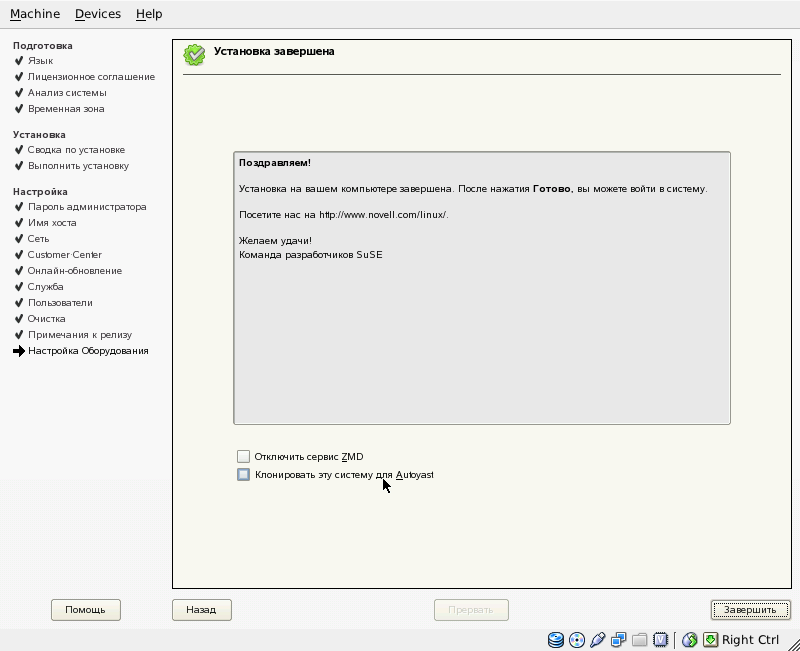
\includegraphics[width=1\linewidth]{oes/15.png}}
\caption{Завершение установки}
\label{fig15}
\end{figure}
Если мы хотим сохранить настройки для будущего клонирования операционной
системы, то ставим крестик в поле <<Клонировать эту систему для Autoyast>>. Жмём кнопку <<Завершить>>.
\clearpage

Теперь мы можем зайти на сервер локально и закончить настройку сервера. (рис.~\ref{fig16})
\begin{figure}[H]
\center{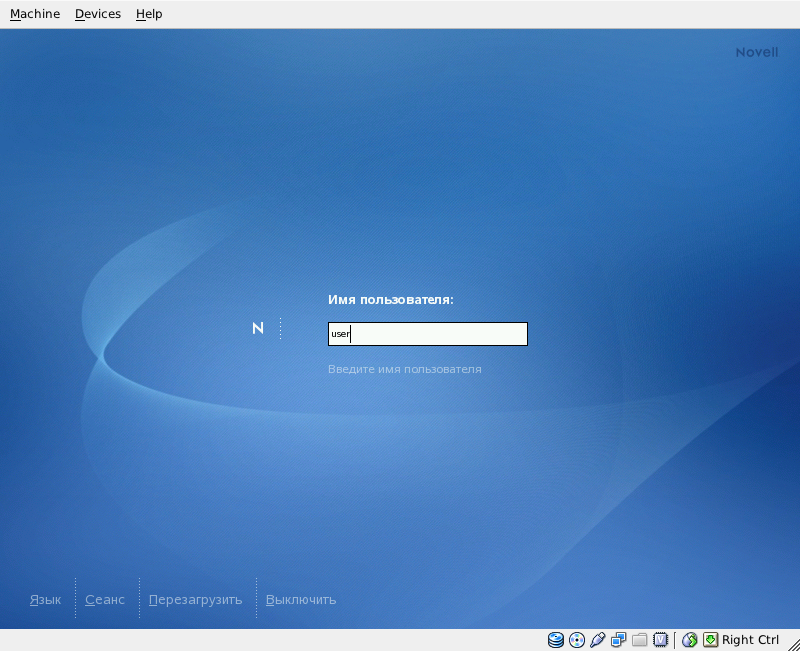
\includegraphics[width=1\linewidth]{oes/16.png}}
\caption{Вход в систему}
\label{fig16}
\end{figure}
\clearpage

\section{Настройка DHCP}
Open Enterprise Server основывается на linux дистрибутиве openSUSE\footnote{http://www.opensuse.org/ru/}, поэтому по вопросам использования или настройки можно воспользоваться любыми справочными материалами, посвящёнными этому дистрибутиву. Здесь мы коснёмся лишь настройке сервисов, относящихся к диску OES2.\par 
Все настройки ОС openSUSE пройзводятся с помощью менеджера YaST\footnote{http://ru.opensuse.org/YaST}.
\begin{figure}[H]
\center{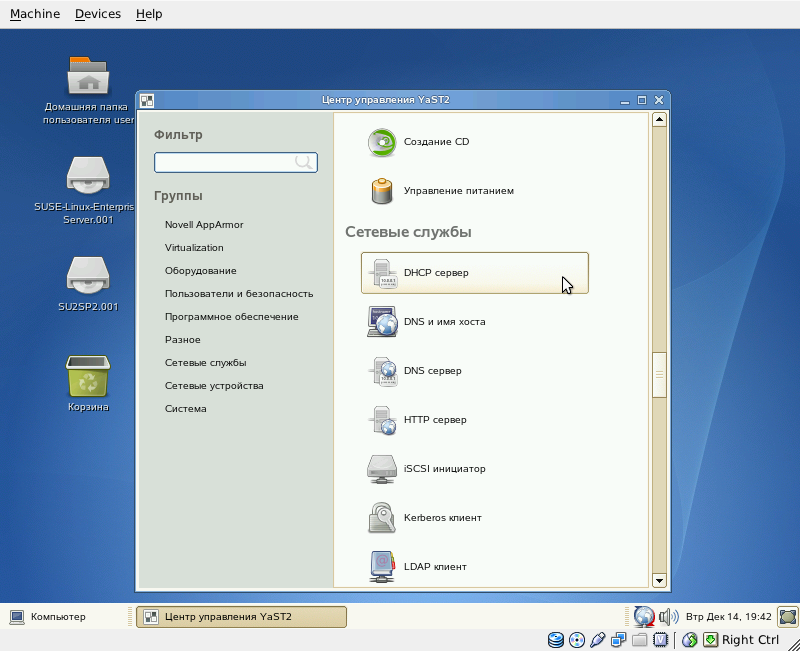
\includegraphics[width=1\linewidth]{oes/yast.png}}
\caption{YaST}
\label{yast}
\end{figure}
Настройка DHCP здесь ничем принципиально не отличается от настройки в Windows системах. Выбирается сетевой интерфейс, на котором будут раздаваться IP адреса, также назначаются сервера имён и диапазон IP адресов. Последний шагом станет выбор, будет ли сервер стартовать при загрузке операционной системы или его следует запускать вручную.\par
В процессе настройки у системы может возникнуть желание доустановить недостающие компоненты. Для этого необходимо вставить соответствующий диск с ПО. Базовые пакеты находятся на дисках SLES, в то время как всё проприетарное программное обеспечение лежит на диске OES2.

\section{Настройка eDirectory}
Настройка eDirectory\footnote{http://www.novell.com/russia/products/edirectory/}
